\documentclass  [12pt]{article}
\usepackage{graphicx}

\author {KARINTHY FRIGYES}
\date{1912   /Így írtok ti/}
\title{Dana Idák*  }

\begin{document}

\begin{titlepage}
    \maketitle
\end{titlepage}




\begin{figure}
\begin{center}
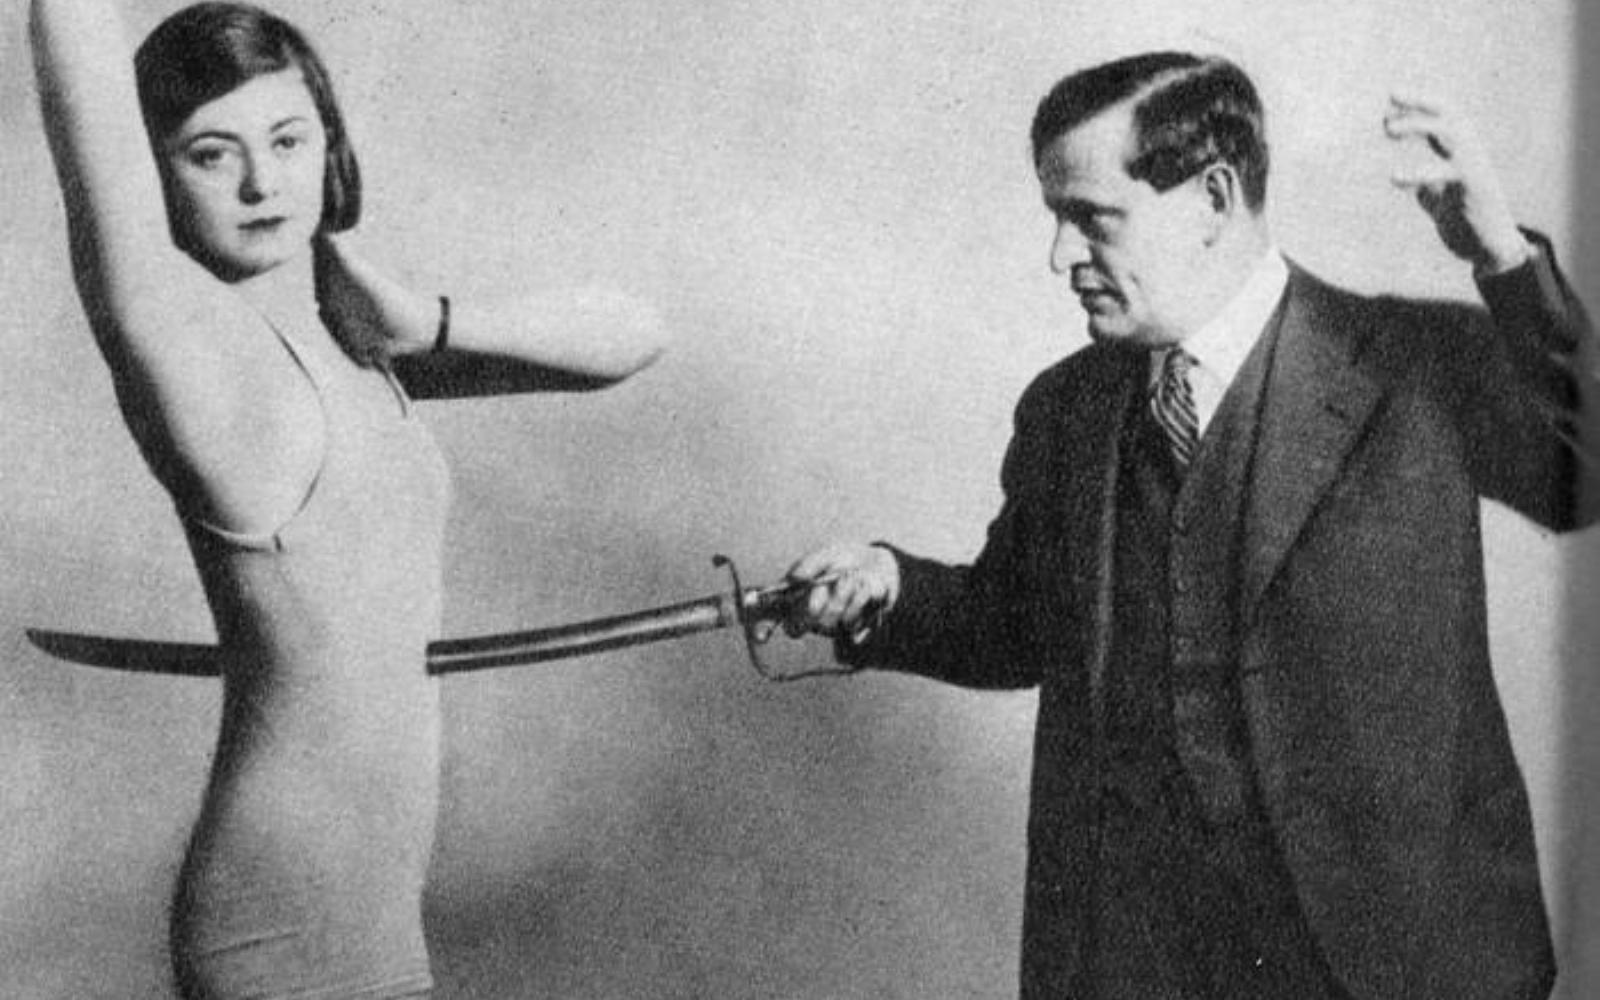
\includegraphics[angle=5, width=5cm]{igy_irtok_ti.jpeg}
\end{center}
\end{figure}


\begin{figure}
\begin{center}
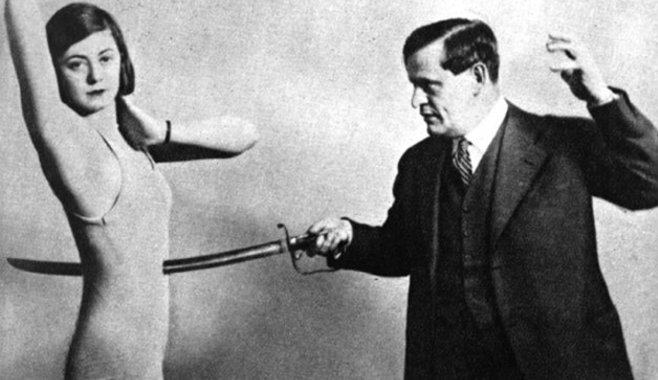
\includegraphics[angle=5, width=5cm]{Frici1.png}
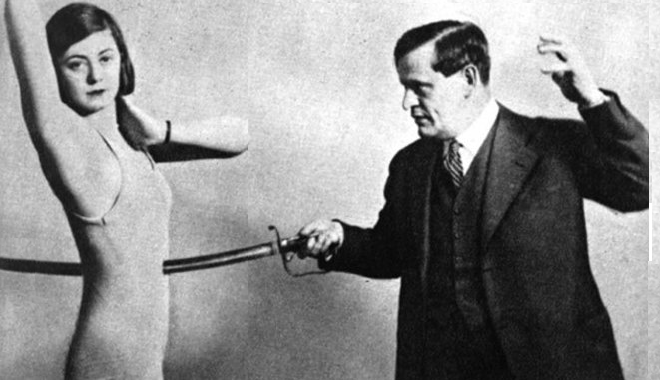
\includegraphics[angle=5, width=5cm]{Frici3.png}
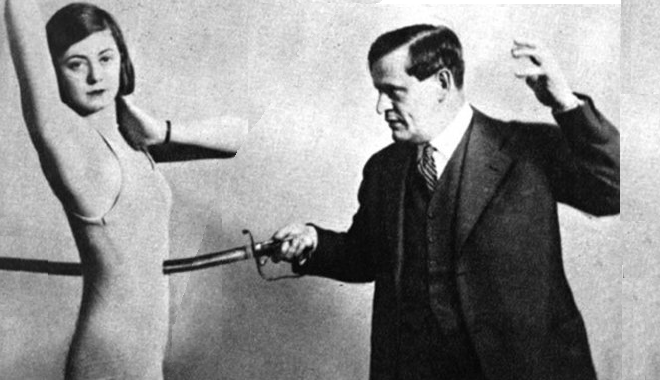
\includegraphics[angle=5, width=5cm]{Frici5.png}
\end{center}
\end{figure}


Lent a lenső lélekuton \{Hádesz öblén, [hol a lélek élet – állott (élet – állott, mint az állat) s aspodélosz illatokkal] öblögetve, ablakokba\} ablakokba öblögetve, öblögekbe ablakogva és makogva mekegve.\\
% a \\ a sortörés jele, nem az új bekezdésé; új bekezdést üres sor után írva lehet indítani
És mekegve és makogva lent a mélybe, lent $ \sqrt[2]{lent}  $ az éjbe, hol a kéjbe $ {ejbe,melybe \choose   kejbe,ejbe} $.
% látom a math mode-ból kivetted az ékezetet, itt így lehet é betűt írni: \acute{e}
% vagy vissza kell váltani text mode-ba a math mode-on belül: ${\mbox{éjbe, mélybe} \choose \mbox{kéjbe, éjbe}}$
% a \choose helyett lehet jobb lenne itt egy \begin{array}
Ötven asszony, logarithmus ötven asszony és emelve és kivonva, négyzetekre köbgyökökre, ötven asszony, hetven asszony, százhuszonhét bűnös asszony, ötven órjás amphorába, asfodélosz ötven asszony = bünös asszony, mennyi jött ki, mennyi jött ki.\\
Százkilencven bűnös asszony, óriási amphorába, amphorába \begin{math} \sqrt[2]{amphoraba} \end{math} , rába, rába, rába, majd mekegve, $(\log) $ majd makogva, mindörökre, mindhiába, (mert hiába [mind hiába] töltögetve, öblögetve) öblögetve ablakokba, ablagokva, és makogva,\begin{displaymath} (oblogekbe)^{2} \end{displaymath} és mekegve és makogva, fogjanak $ \sqrt[2]{fogjanak} $ meg, fogjanak meg…\\

\begin{center}
(Megfogják.)
\end{center}

\tiny *Matematikai költemény.
% ha ez a címnek a lábjegyzete, akkor arra a \footnote{Matematikai költemény.} a legmegfelelőbb


\end{document}
